\chapter{Ideal integral (PI) controller design}

\section{Specifying the problem}
An ideal integral controller improves the steady-state error of the system. For a step input, the error is proven to be 0 in the previous chapter. Therefore, it is of interest to improve the error of a ramp input by designing an active controller. The design problem is

\textbf{Design an active controller to yield $ 10\% $ overshoot and zero stead-state error for a ramp input.}

\section{Solving the problem}
Using the results from the previous chapter, the closed-loop poles $ s = -2.5 \pm j3.411 $ are used to find the appropriate zero in the ideal integral fraction $ (s+z_c)/s $. Arbitrarily choose $ z_c = 0.1 $ and compare if the gain $ K $ is closed to the previous value $ K_p = 0.9827 $. Using $ s = -2.5 + j3.411 $ as the value for calculation, the angle is
\[
\begin{array}{ll}
\theta & = \angle (s+0.1) - 2[\angle (s+0)] - \angle (s+5)\\
& = \angle (-2.5+j3.411+0.1) - 2[\angle (-2.5+j3.411+0)] - \angle (-2.5+j3.411+5)\\
& = 125.13^\circ - 2\times 126.24^\circ - 53.76^\circ\\
& = -181.11^\circ \approx -180^\circ\\
\end{array}
\]
which is near the root locus but does not significantly affect the transient response. The corresponding gain is
\[
\begin{array}{ll}
K & = \dfrac{|s|}{|s+0.1|}\dfrac{|s||s+5|}{18.2}\\
& = \dfrac{|-2.5 + j3.411|}{|-2.5 + j3.411+0.1|}\dfrac{|-2.5 + j3.411||-2.5 + j3.411+5|}{18.2} \\
& = 0.996 \approx 1\\
\end{array}
\]

Thus, the transfer function for the ideal integral controller is
\begin{equation}
	G_c(s) = K\dfrac{s+0.1}{s} = 0.996 + \dfrac{0.1}{s}
\end{equation}

In summary, the proportional gain is $ K_p = 1 $ and integral gain is $ K_i = 0.1 $. From the figure, the response uses an active PI controller converges to ramp input, which satisfies the requirement.

\section{Graphic results}
\subsection{Transfer function of PI controller}
\begin{minted}{python}
	from control import *
	from numpy import *
	from matplotlib.pyplot import *
	
	
	s = tf('s')
	G = tf([18.2],[1,5,0])
	rlocus(G)
	
	zeta = -log(0.1) / sqrt(pi**2 + log(0.1)**2)
	x = array([-10,0])
	
	plot(x, tan(pi-arccos(zeta))*x)
	print(0.996*array([1,0.1]))
\end{minted}
\begin{figure}[ht]
	\centering
	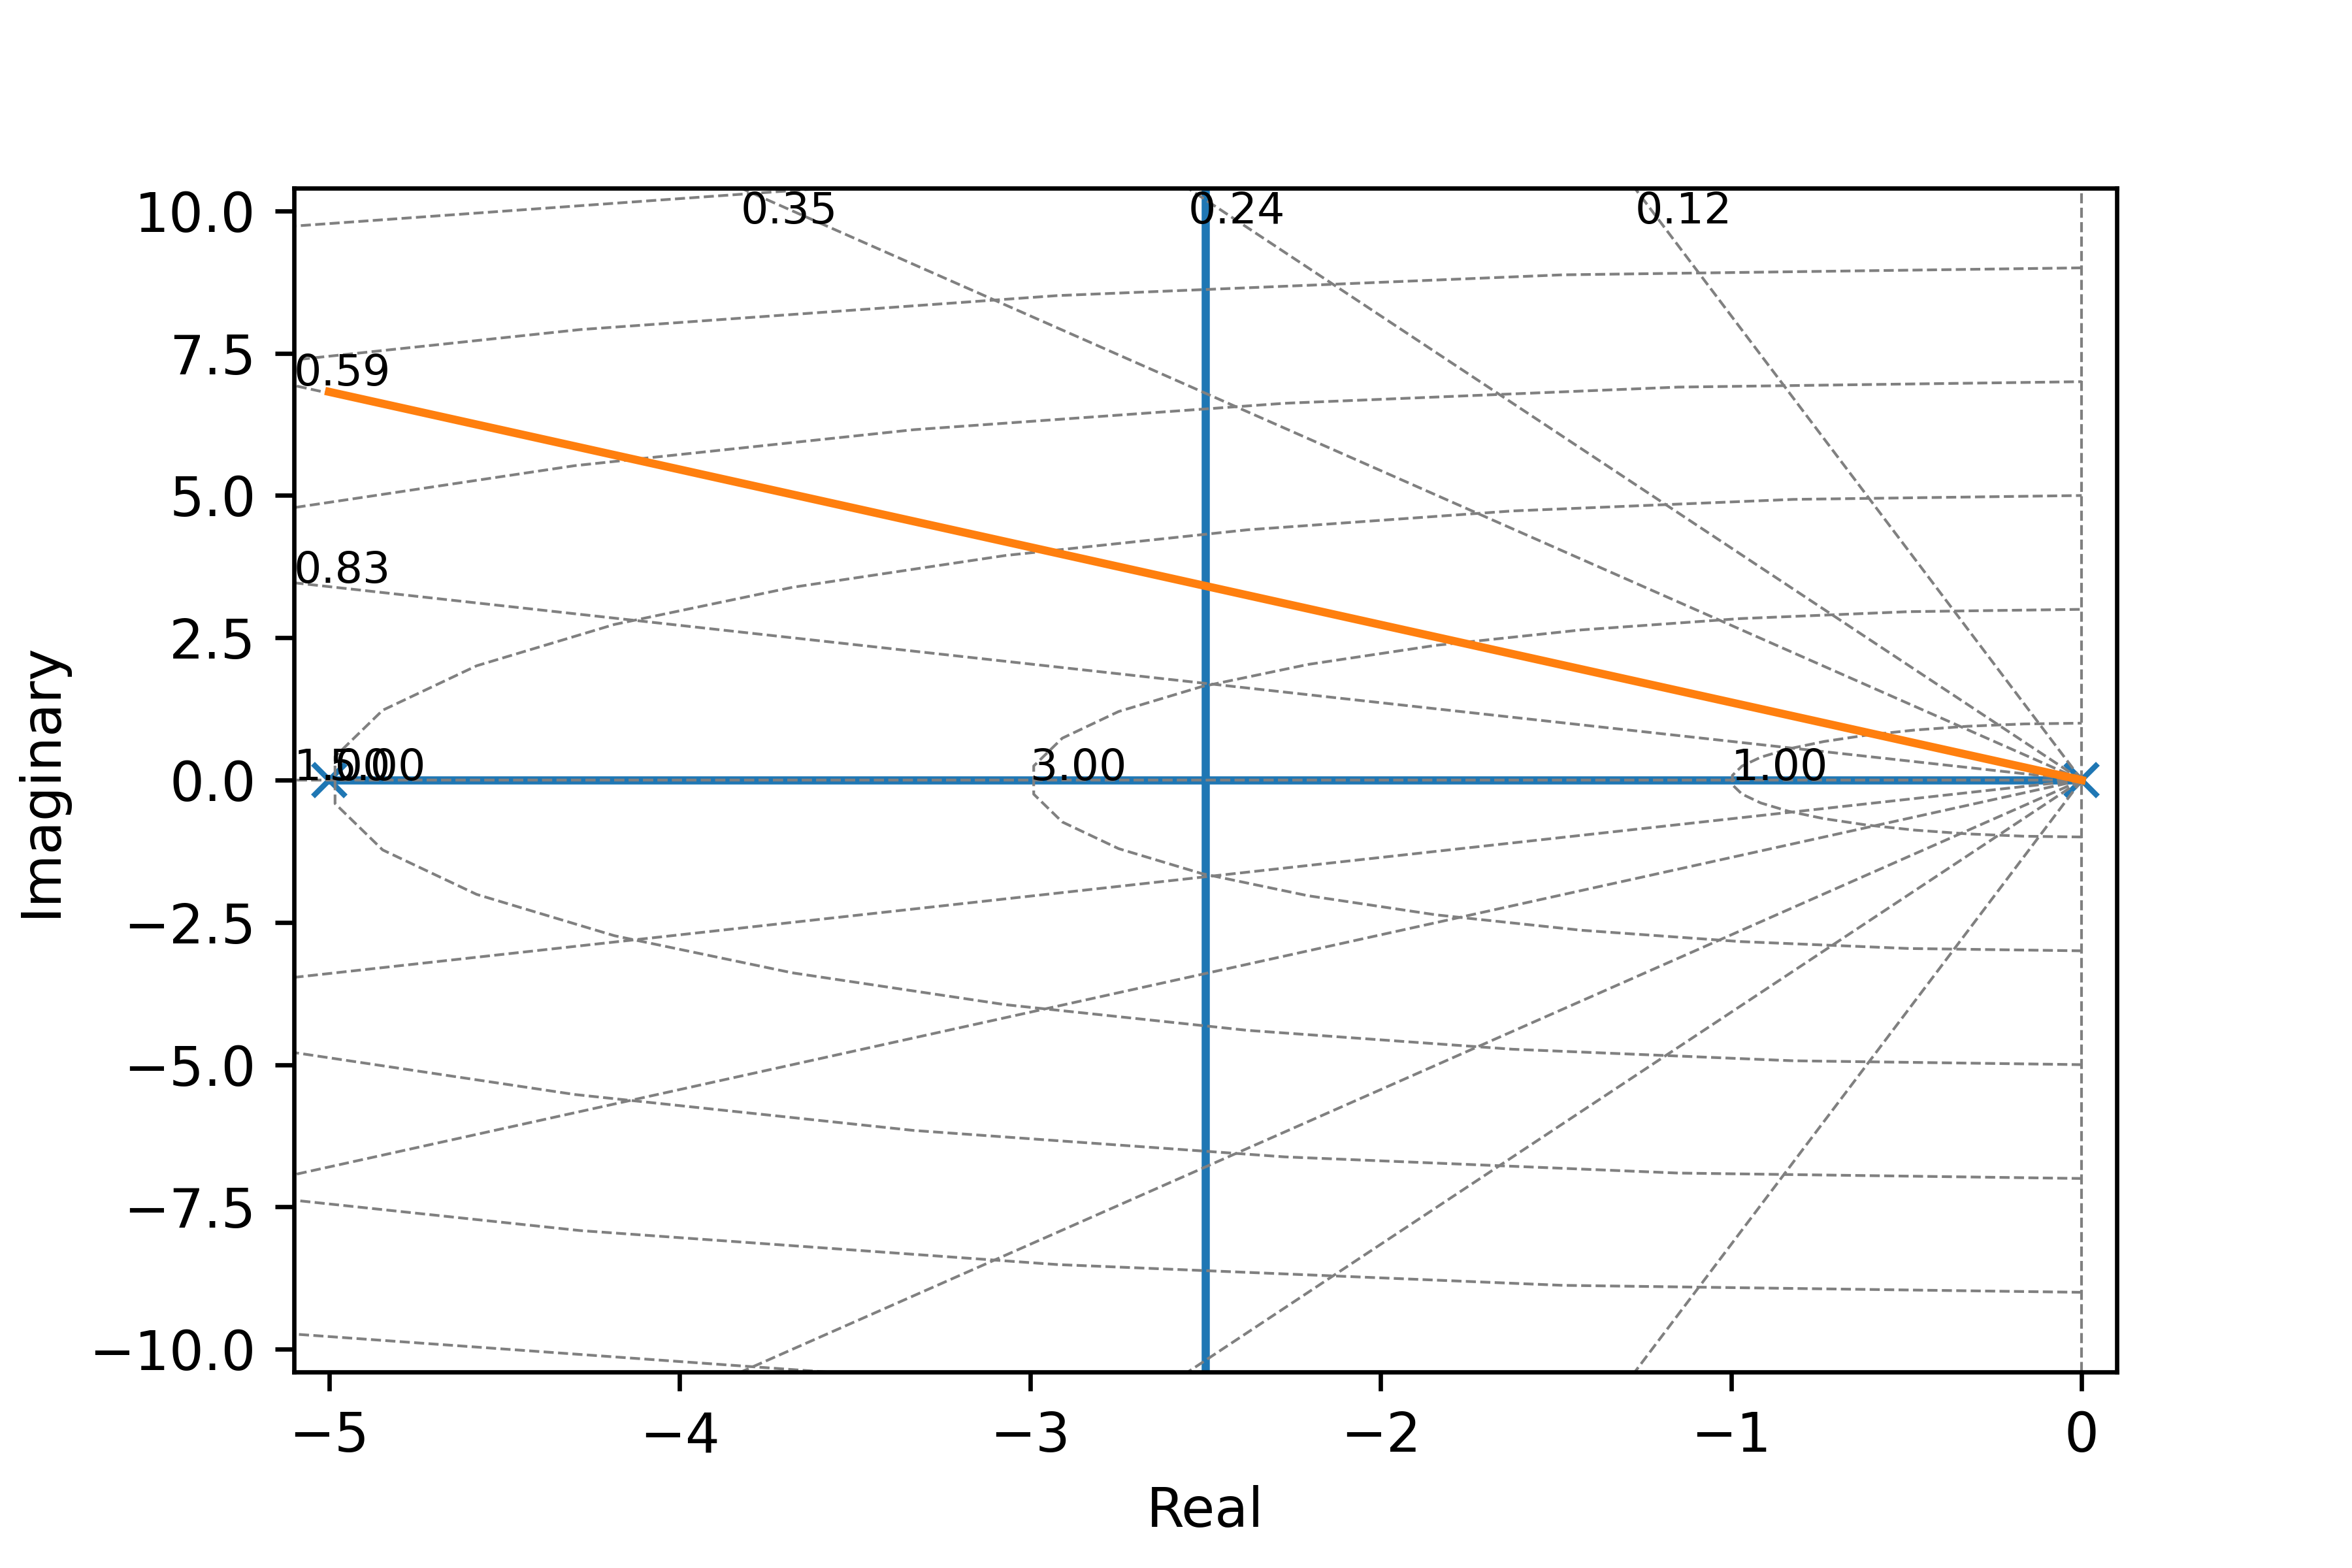
\includegraphics[width=0.7\linewidth]{rlocus}
	\caption{Root locus of the open-loop uncompensated system}
\end{figure}


\subsection{Transient response of the system}
\subsubsection{Step response}
\begin{minted}{python}
	from control import *
	from numpy import *
	from matplotlib.pyplot import *
	
	
	s = tf('s')
	G = tf([18.2],[1,5,0]) * (1+0.1/s)
	sys = feedback(0.996*G, 1)
	
	T = linspace(0,5,1000)
	
	plot(*step_response(sys, T=T))
\end{minted}
\begin{figure}[ht]
	\centering
	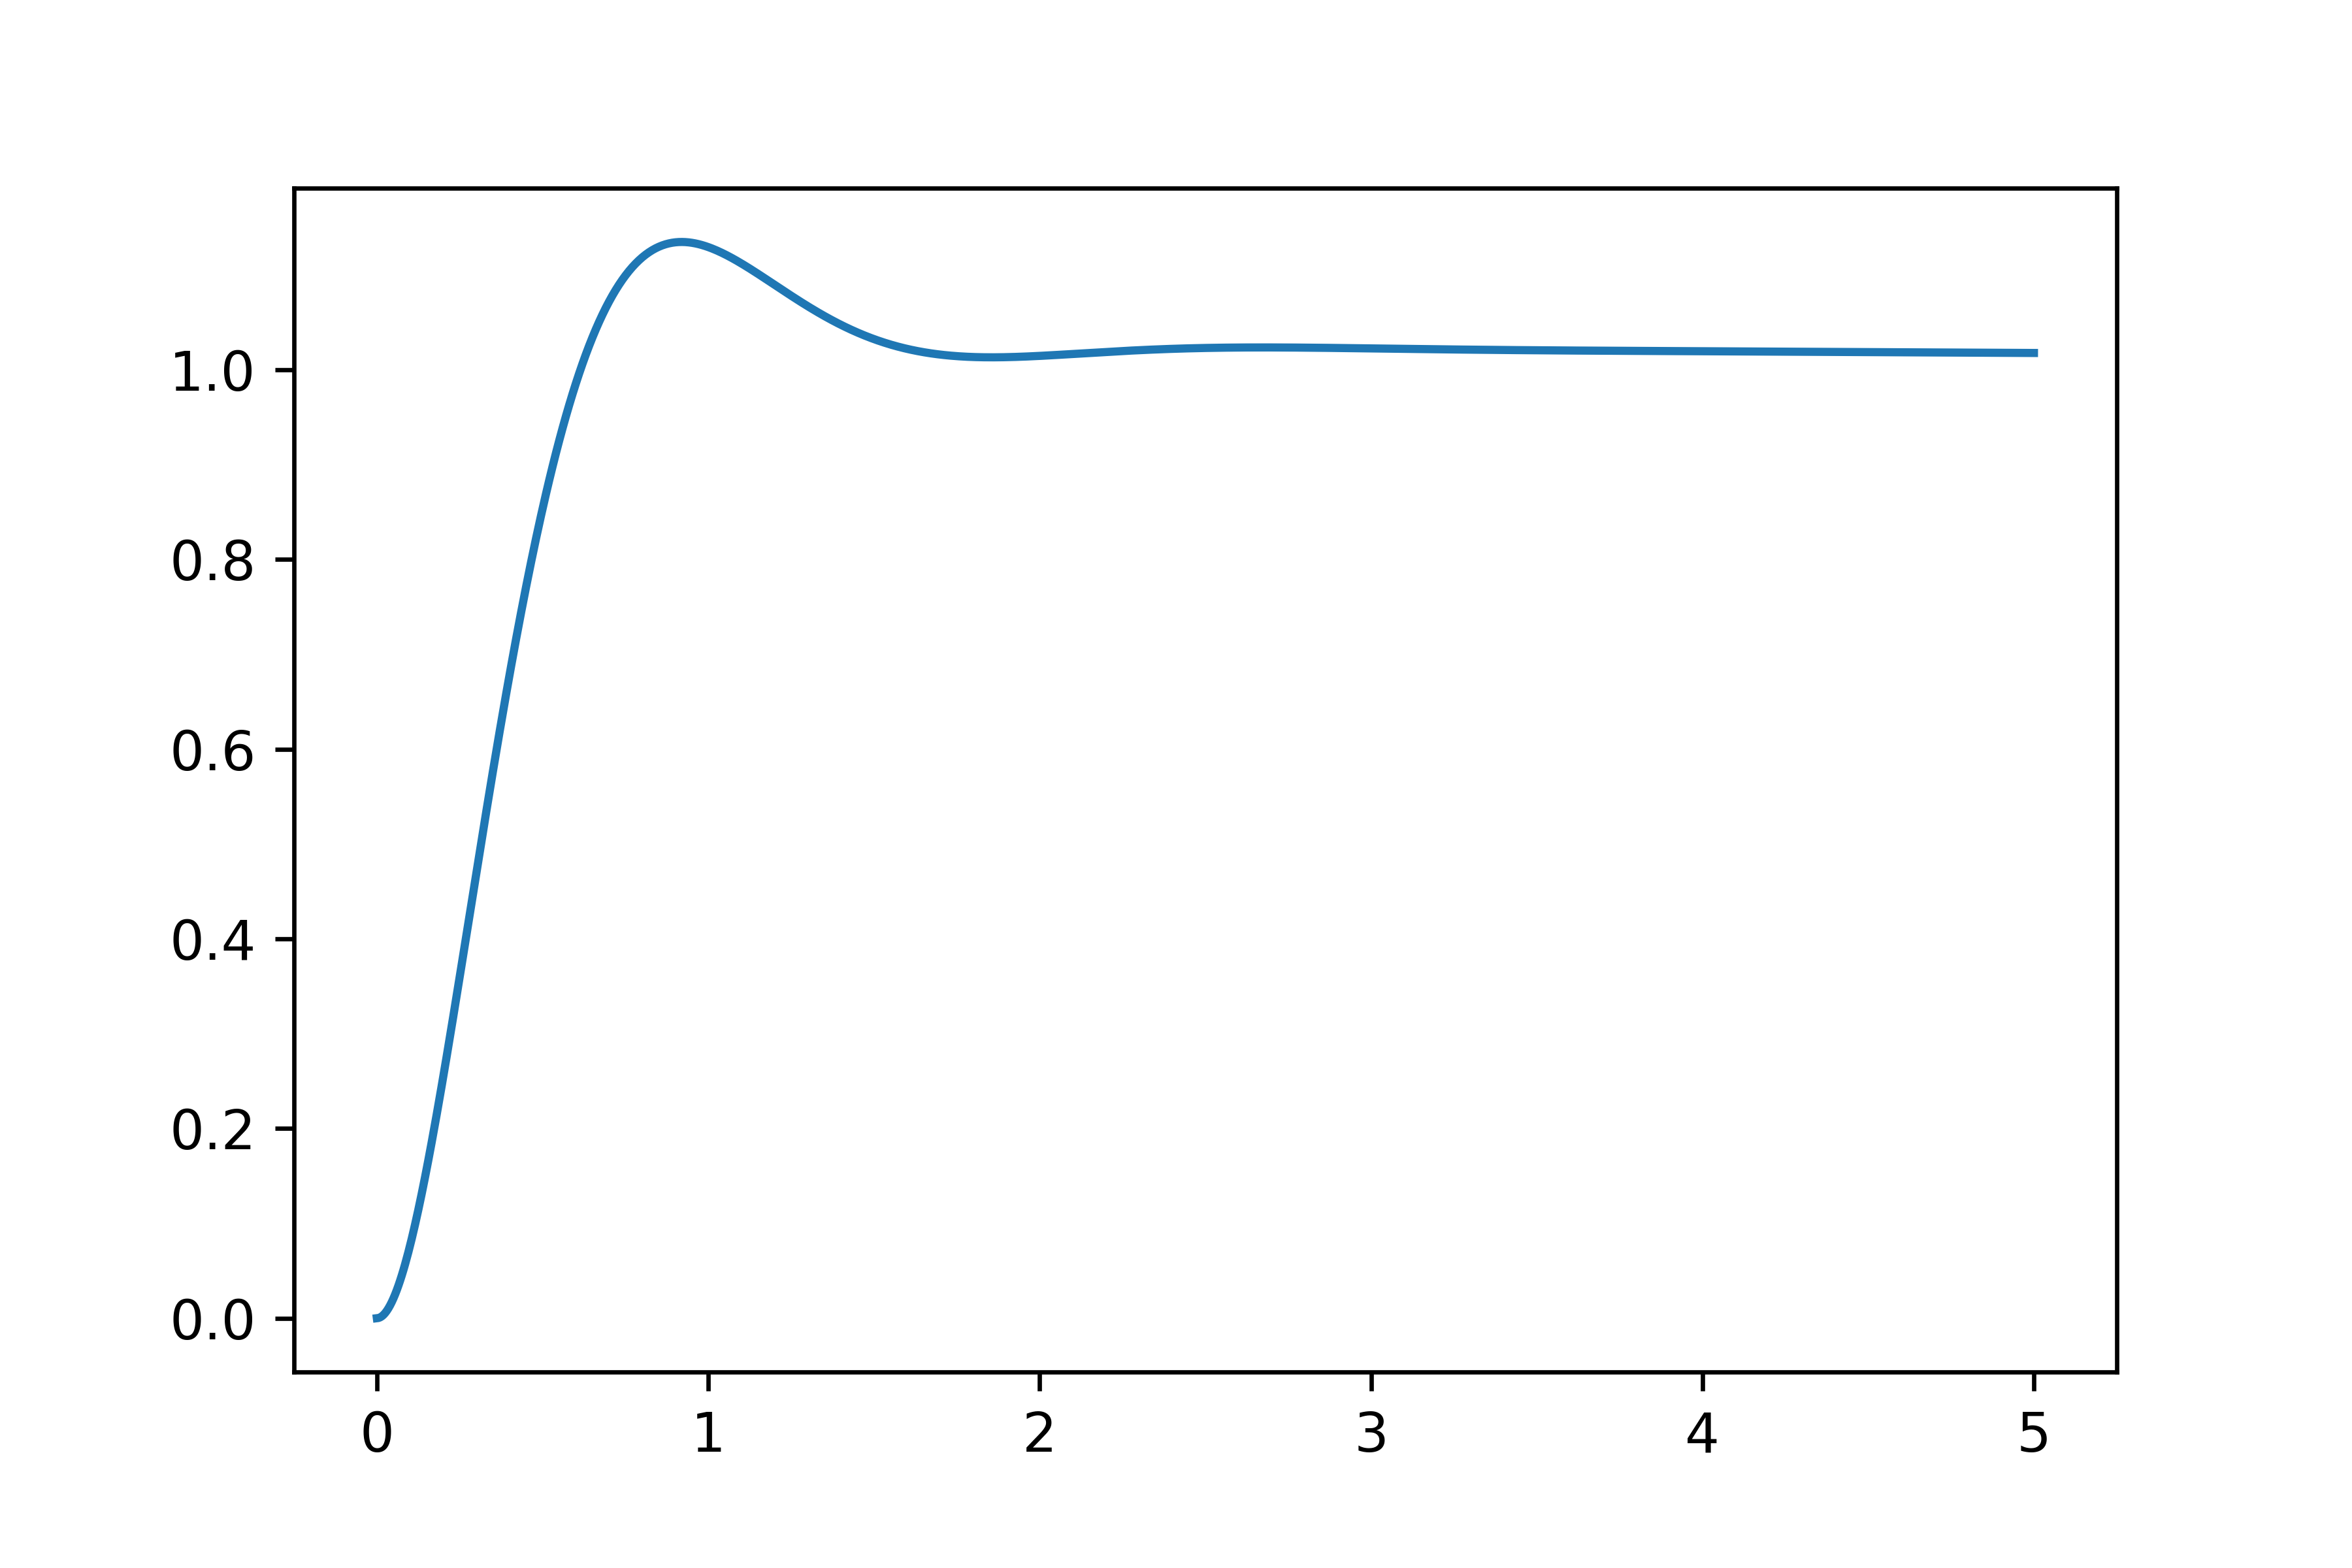
\includegraphics[width=0.7\linewidth]{step_pi}
	\caption{Step response of the system using PI controller}
\end{figure}

\subsubsection{Ramp response}
\begin{minted}{python}
	from control import *
	from numpy import *
	from matplotlib.pyplot import *
	
	
	s = tf('s')
	G = tf([18.2],[1,5,0]) * (1+0.1/s)
	sys = feedback(0.996*G, 1)
	
	U = T = linspace(0, 2, 1000)
	yout, T, xout = lsim(sys, U, T)
	
	plot(T, U, color='gray', label='ramp input')
	plot(T, yout, color='blue', label='ramp response')
	legend()
\end{minted}
\clearpage
\begin{figure}[ht]
	\centering
	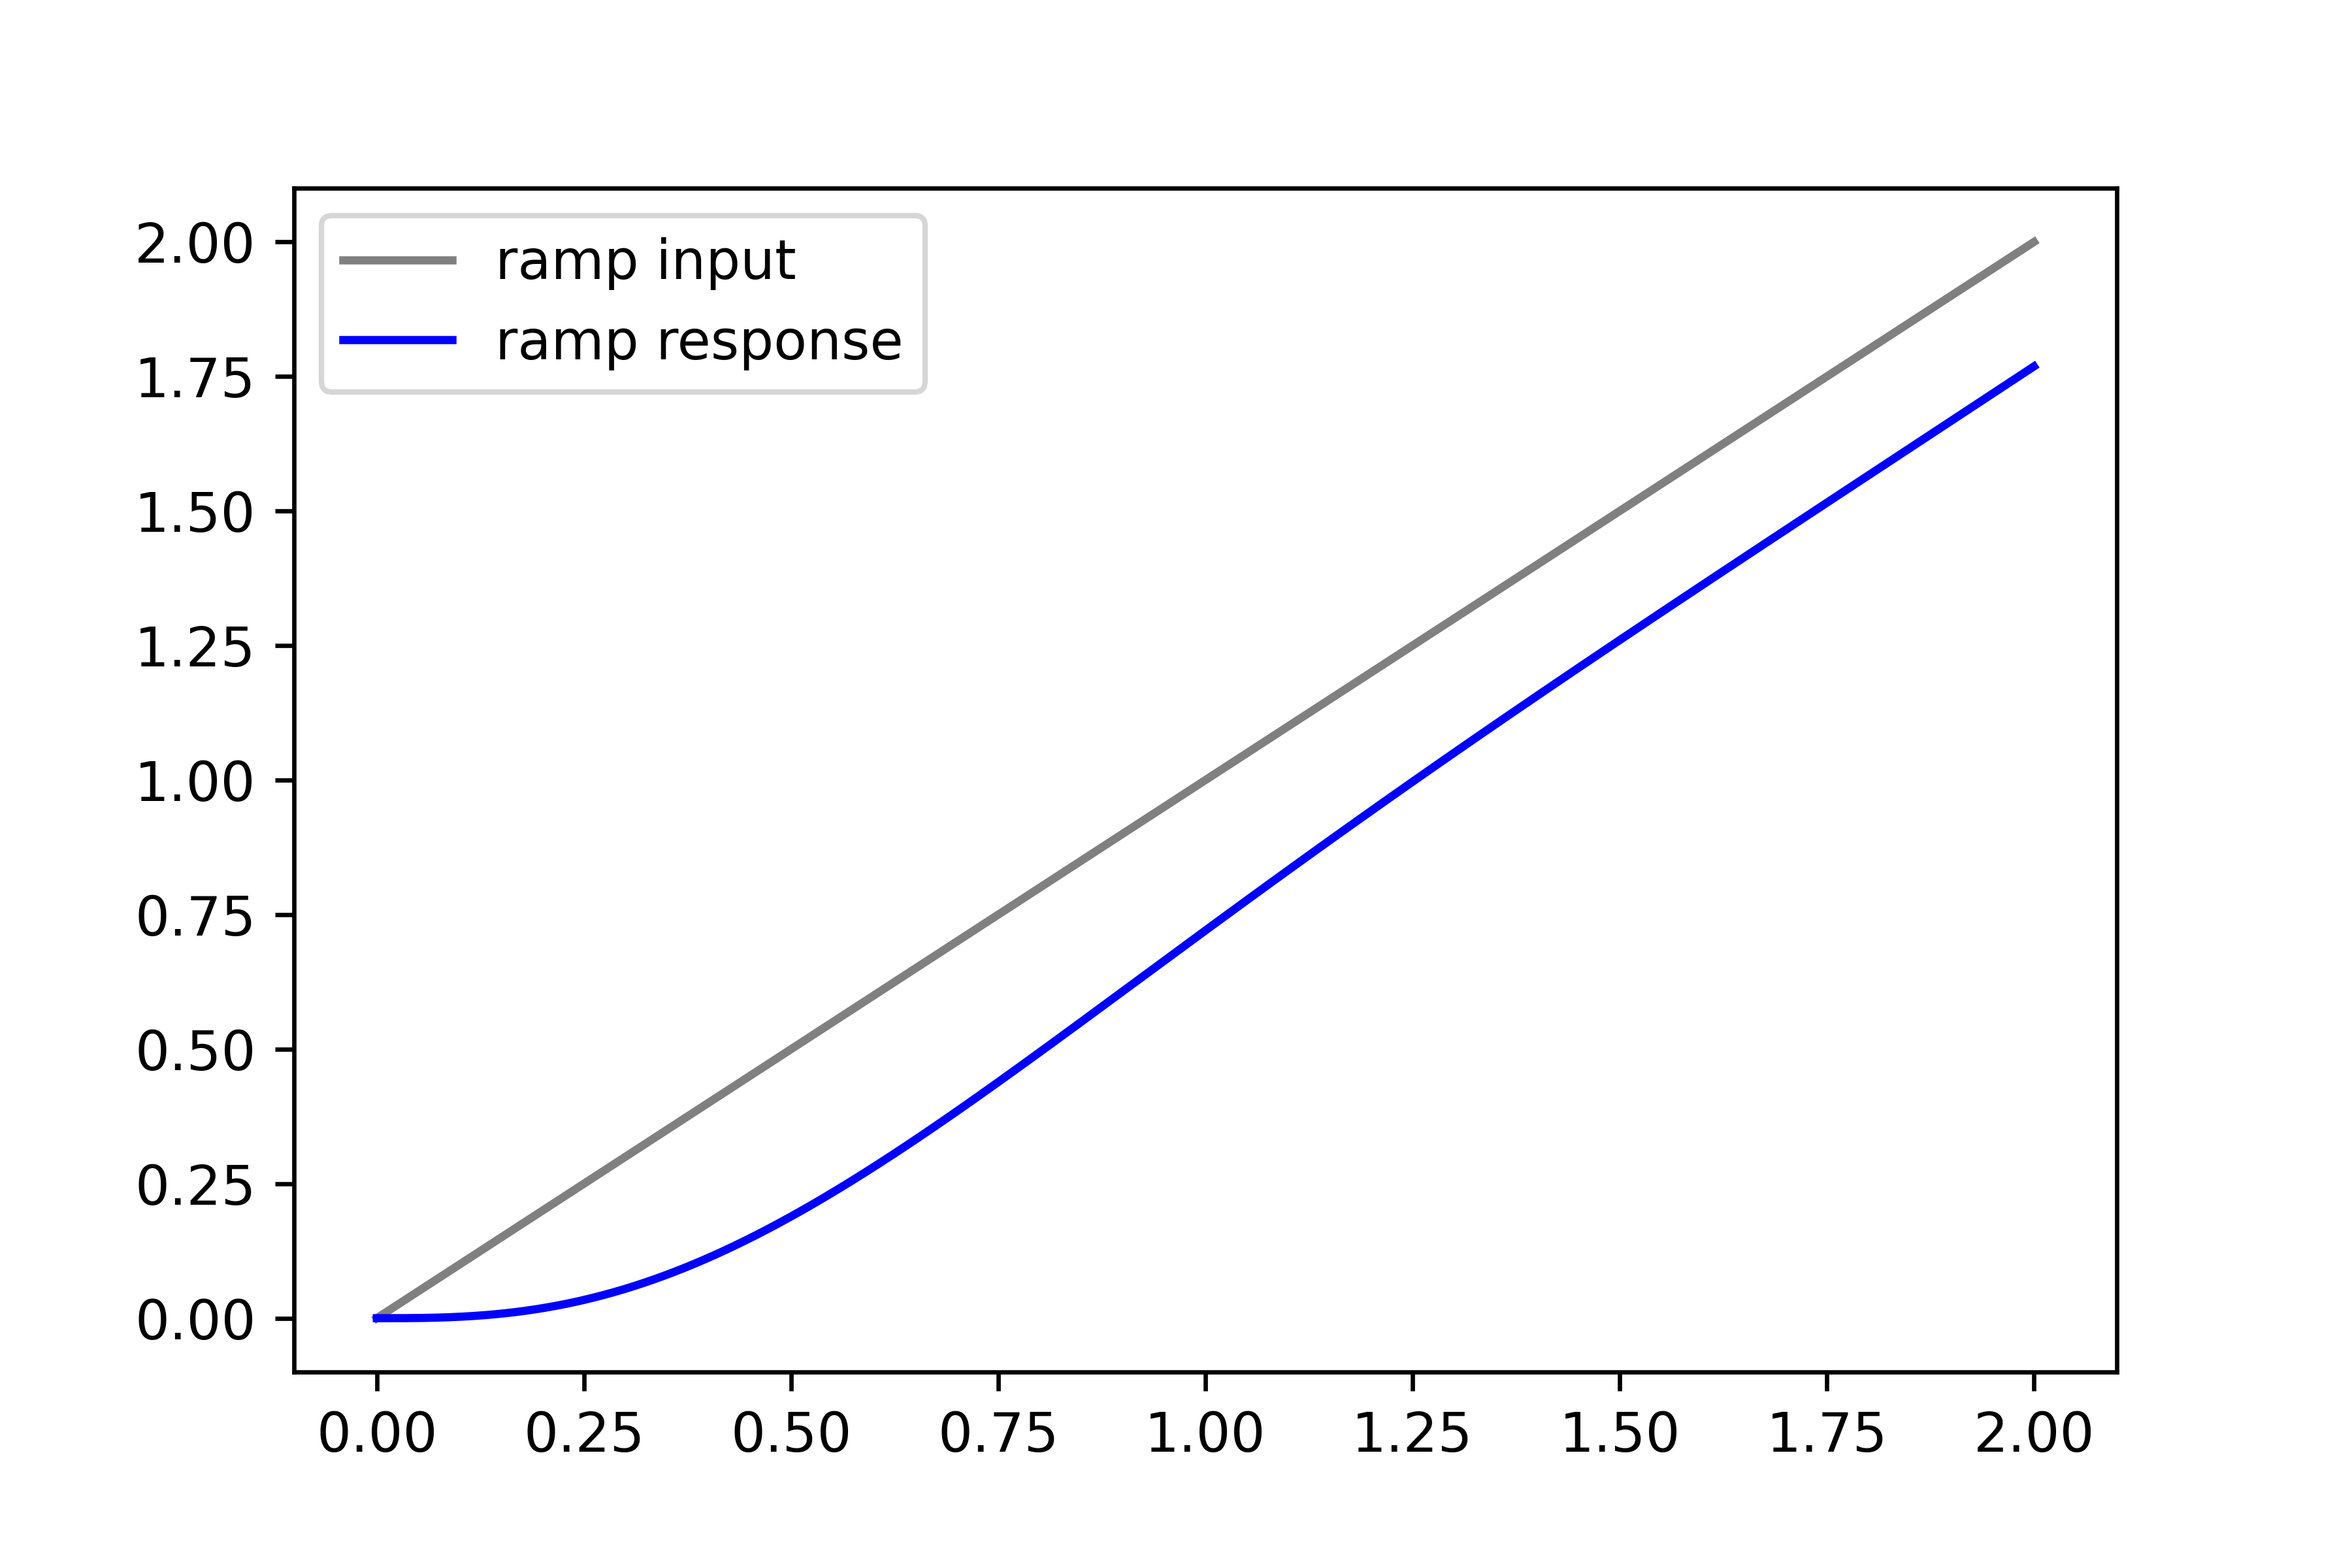
\includegraphics[width=0.7\linewidth]{ramp_pi}
	\caption{Ramp response of the system using PI controller}
\end{figure}